\documentclass[11pt]{article}
\usepackage[a4paper,margin=22mm]{geometry}
\usepackage{amsmath,graphicx,booktabs,hyperref}
\newcommand{\TrainingCount}{240}
\newcommand{\ValidationCount}{9391}
\newcommand{\AcceptedCount}{9390}
\newcommand{\FallbackCount}{1}
\newcommand{\WorstError}{0.00903}
\newcommand{\WorstCharge}{3.829}
\newcommand{\RefinementError}{0.0000350}
\newcommand{\ModelMilliseconds}{2.05}
\newcommand{\PilotCount}{100}
\newcommand{\PilotFastPads}{138}
\newcommand{\PilotSpicePads}{469}
\newcommand{\PilotLinearPads}{8460}
\newcommand{\PilotFastError}{0.00655}
\newcommand{\PilotFastCharge}{0.741}
\newcommand{\PilotAllError}{0.4154}
\newcommand{\PilotAllCharge}{199.018}
\newcommand{\PilotMeanCharge}{-53.175}
\newcommand{\PilotMaxPulse}{0.096}
\newcommand{\NonlinearSeconds}{3.83}
\newcommand{\WorkflowSeconds}{104.0}
\newcommand{\DomainExcursion}{0.675908}
\newcommand{\DomainCurrent}{77.798}

\title{ITACA: fast nonlinear CSA response}
\author{Generated from Julia validation results}\date{2026-11-05}
\begin{document}\maketitle
\section{Model and domain}
The state $x=V_0-V_{\mathrm{out}}$ follows
\[\dot{x}=g(x)I(t)/e-r(x),\qquad x(0)=0.\]
The gain $g$ (V per elementary charge) and recovery $r$ (V/s) are continuous
piecewise-linear tables fitted to \TrainingCount{} saved SPICE histories.
Recovery vanishes at equilibrium. Each prediction follows the complete current
history from baseline, including the quiet tail. RK4 steps end at current knots
and acquisition-window boundaries, with a maximum step of $100\,\mu$s.
The calibrated excursion extends to \DomainExcursion{} V and current to
\DomainCurrent{} fA, for the existing $0.5$ mm square pad, $5$ mm final gap,
$3$ m/s gap velocity and uniform mean arrivals within each frame.
The existing 5 ms voltage average, three-frame inverse and stationary
Gaussian temporal noise covariance are retained. The guard remains 0.63 V.
Controls and out-of-domain histories use SPICE.
\section{Independent validation}
Calibration and validation use disjoint event IDs. Of \ValidationCount{}
held-out histories, \AcceptedCount{} lie inside the calibration domain and
\FallbackCount{} requires SPICE. The worst corrected-bucket error is
\WorstError{} ENC against the 0.5 ENC criterion. The largest event-total
difference is \WorstCharge{} ions. Halving the integration step changes the
corrected estimates by at most \RefinementError{} ENC. Median model runtime
is \ModelMilliseconds{} ms per history on this machine.
\begin{center}\small\begin{tabular}{rrrrrr}\toprule
Frame (ms)&Histories&Fallbacks&Max (ENC)&Median (ENC)&Runtime (ms)\\\midrule
20 & 502 & 1 & 0.00454 & 0.00150 & 1.99 \\
30 & 2898 & 0 & 0.00547 & 0.00089 & 2.17 \\
40 & 5991 & 0 & 0.00903 & 0.00077 & 2.02 \\
\bottomrule\end{tabular}
\end{center}
\begin{figure}[ht]\centering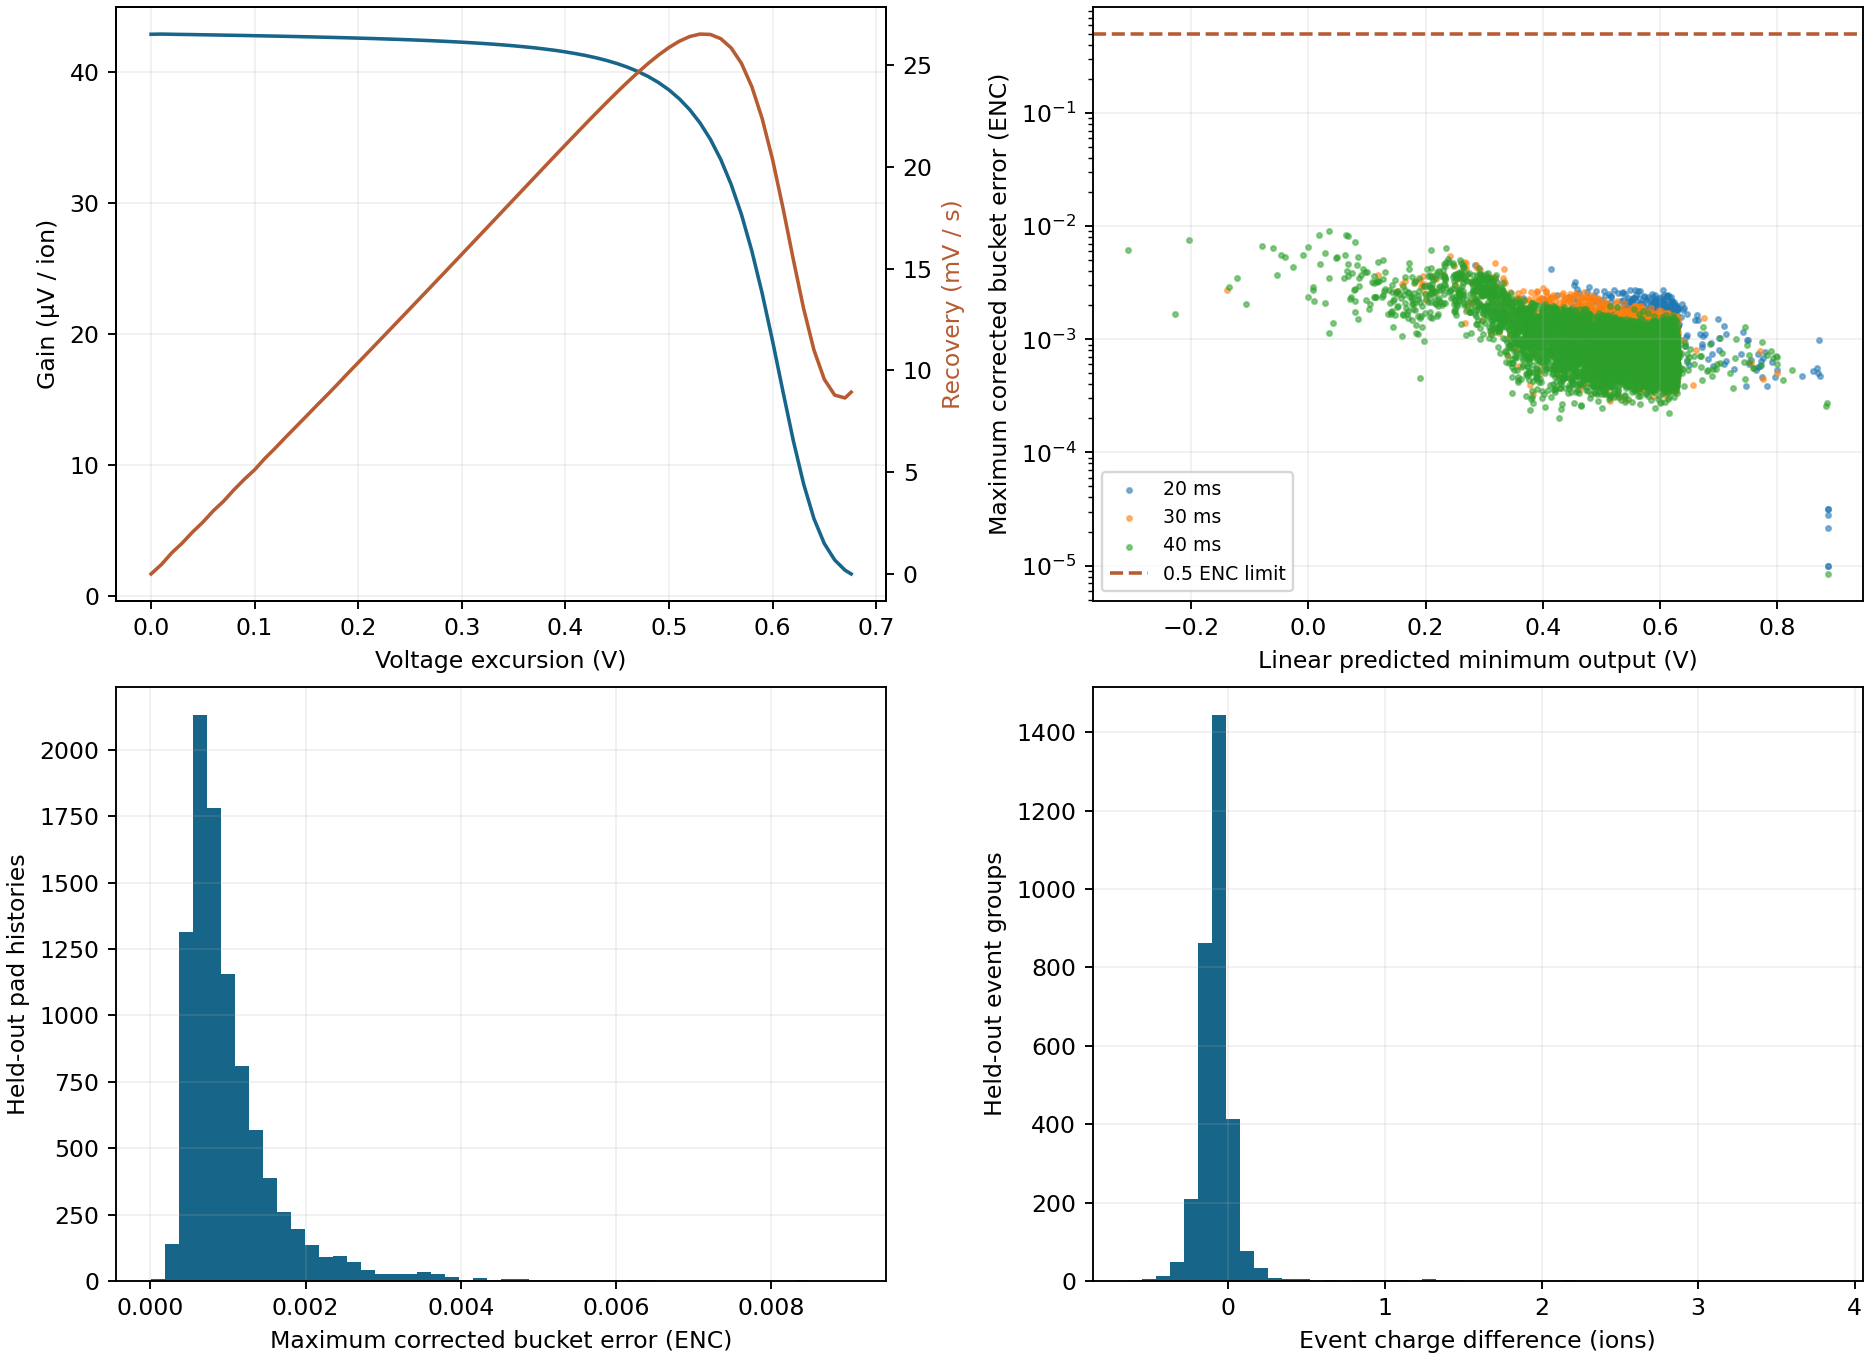
\includegraphics[width=\linewidth]{validation.png}
\caption{Fitted response and held-out validation. Event totals replace only
below-guard histories inside the domain; unchanged linear and fallback SPICE
histories cancel.}\end{figure}
\clearpage\section{End-to-end production pilot}
The \PilotCount{}-event 4 mm pilot has \PilotLinearPads{} linear,
\PilotFastPads{} fast nonlinear and \PilotSpicePads{} SPICE-control histories.
The nonlinear replacement alone differs from saved SPICE by at most
\PilotFastError{} ENC per bucket and \PilotFastCharge{} ions per event.
The nonlinear evaluation stage, including control predictions, took
\NonlinearSeconds{} s. The filtered workflow took \WorkflowSeconds{} s after
preparation, including startup, SPICE controls, solver refinement and reduction.
These timings do not include input preparation or the later correction and
publication stages; they are not a full-production speedup measurement.

The smaller pilot selects different above-guard SPICE controls from the
original 8,000-event run. Including that selection change gives a maximum
bucket difference of \PilotAllError{} ENC, maximum event-charge difference
\PilotAllCharge{} ions and mean difference \PilotMeanCharge{} ions.
The maximum-pulse difference is \PilotMaxPulse{} ions. The model-only metric
isolates the nonlinear replacement. A common noise draw isolates response
differences; new production identities otherwise have independent deterministic
noise draws. Signed estimates, quiet buckets, covariance and ion ledgers pass
the existing production checks.
\begin{figure}[ht]\centering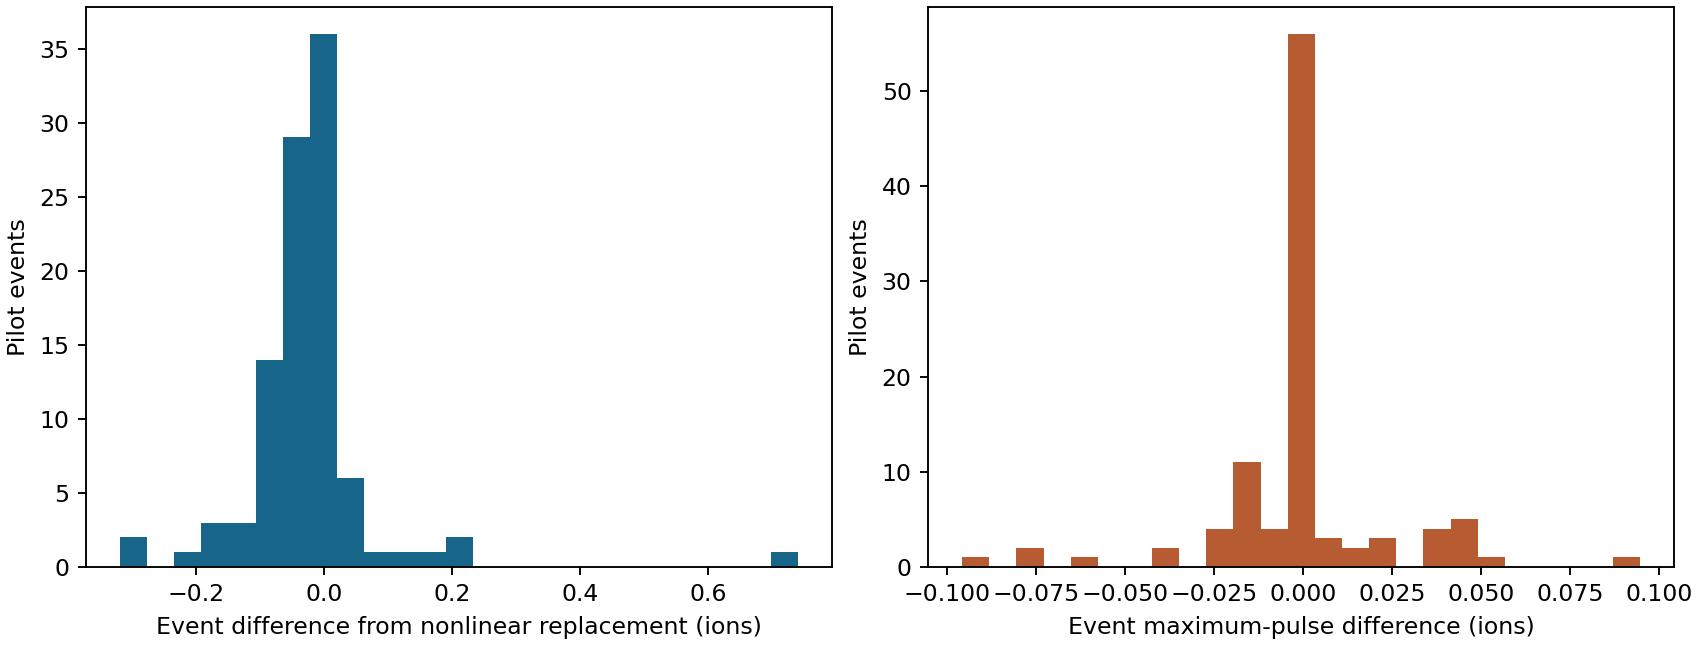
\includegraphics[width=\linewidth]{pilot.png}
\caption{Model-only charge differences and complete-pipeline maximum-pulse differences.}\end{figure}
\section{Production and provenance}
New production defaults to \texttt{hybrid\_nonlinear}. An explicit
\texttt{response\_model = "hybrid\_spice"} selects the reference backend.
HDF5 model codes are 0 linear, 1 SPICE and 2 calibrated nonlinear.
Calibration content, circuit and model code are checked and hashed into
the resolved run identity. Numerical results and source hashes are in
\path{results/ion_csa_nonlinear/v1/}. Reproduce the pilot with
\texttt{make ion-csa-nonlinear-pilot}, and regenerate this report with
\texttt{make ion-csa-nonlinear-report}. The numerical calibration is a local
HDF5 artifact regenerated by the calibration script and its TOML card.
\end{document}
